\documentclass[runningheads]{llncs}

% ---------------------------------------------------------------
% Include basic ECCV package
 
% TODO REVIEW: Insert your submission number below by replacing '*****'
% TODO FINAL: Comment out the following line for the camera-ready version
\usepackage[review,year=2026,ID=5]{eccv}
% TODO FINAL: Un-comment the following line for the camera-ready version
%\usepackage{eccv}

% OPTIONAL: Un-comment the following line for a version which is easier to read
% on small portrait-orientation screens (e.g., mobile phones, or beside other windows)
%\usepackage[mobile]{eccv}


% ---------------------------------------------------------------
% Other packages

% Commonly used abbreviations (\eg, \ie, \etc, \cf, \etal, etc.)
\usepackage{eccvabbrv}

% Include other packages here, before hyperref.
\usepackage{graphicx}
\usepackage{booktabs}

% additions
% addition
\usepackage{graphicx}
\usepackage{subcaption}
% \usepackage{amsmath}
\DeclareMathOperator*{\argmax}{arg\,max}
\usepackage{multirow}
\usepackage{graphicx}
\usepackage{svg}
\usepackage{arydshln}
\usepackage{nicematrix}
\usepackage{algorithm}
\usepackage{algorithmic}
\usepackage{todonotes}
\usepackage[normalem]{ulem}
\useunder{\uline}{\ul}{}
\usepackage{amsfonts}
\usepackage{color}
\usepackage{comment}

% \newtheorem{proposition}{Proposition}
% \newtheorem{remark}{Remark}

\newcommand{\commentVahidin}[1]{\textcolor{blue}{[Vahidin comment: #1]}} 
\newcommand{\commentSenka}[1]{\textcolor{red}{[Senka comment: #1]}} 
\newcommand{\commentAmar}[1]{\textcolor{green}{[Amar comment: #1]}}

% The "axessiblity" package can be found at: https://ctan.org/pkg/axessibility?lang=en
\usepackage[accsupp]{axessibility}  % Improves PDF readability for those with disabilities.


% ---------------------------------------------------------------
% Hyperref package

% It is strongly recommended to use hyperref, especially for the review version.
% Please disable hyperref *only* if you encounter grave issues.
% hyperref with option pagebackref eases the reviewers' job, but should be disabled for the final version.
%
% If you comment hyperref and then uncomment it, you should delete
% main.aux before re-running LaTeX.
% (Or just hit 'q' on the first LaTeX run, let it finish, and you
%  should be clear).

% TODO FINAL: Comment out the following line for the camera-ready version
%\usepackage[pagebackref,breaklinks,colorlinks,citecolor=eccvblue]{hyperref}
% TODO FINAL: Un-comment the following line for the camera-ready version
\usepackage{hyperref}

\usepackage{graphicx}
\graphicspath{{figures/}}
\usepackage{amsmath,amssymb}
\usepackage{booktabs}
\usepackage{multirow}
\usepackage{xcolor}
\usepackage{microtype}
\usepackage{tikz}
\usetikzlibrary{positioning, arrows.meta}

% Compact float/table spacing to stay within the page budget (layout only, no content lost)
\setlength{\textfloatsep}{7pt plus 2pt minus 2pt}
\setlength{\intextsep}{7pt plus 2pt minus 2pt}
\renewcommand{\arraystretch}{0.96}
% Set the reference list in a slightly smaller font with tight spacing (applied inside the list so llncs does not override it)
\makeatletter
\let\@stdthebibliography\thebibliography
\renewcommand{\thebibliography}[1]{\@stdthebibliography{#1}\footnotesize\setlength{\itemsep}{1pt plus 0.2pt}\setlength{\parsep}{0pt}}
\makeatother

% Convenience macros for placeholders
\newcommand{\TBD}[1]{\textcolor{red}{\textbf{[TBD: #1]}}}
\newcommand{\TODO}[1]{\textcolor{blue}{\textbf{[TODO: #1]}}}
\newcommand{\numimages}{200}      % update when dataset is fixed
\newcommand{\numactions}{6}
\newcommand{\numllms}{4}        % standard VLMs in the agreement pool; o4-mini is evaluated separately

% Support for ORCID icon
\usepackage{orcidlink}


\begin{document}

% ---------------------------------------------------------------
% TODO REVIEW: Replace with your title
\title{Can Frontier Vision-Language Models Reason About the Interactable World? A Typed Affordance Evaluation}

% TODO REVIEW: If the paper title is too long for the running head, you can set
% an abbreviated paper title here. If not, comment out.
% \titlerunning{Effects of model quantization on MLLM explanations}

% TODO FINAL: Replace with your author list. 
% Include the authors' OCRID for the camera-ready version, if at all possible.
\author{First Author\inst{1}\orcidlink{0000-1111-2222-3333} \and
Second Author\inst{2,3}\orcidlink{1111-2222-3333-4444} \and
Third Author\inst{3}\orcidlink{2222--3333-4444-5555}}

% TODO FINAL: Replace with an abbreviated list of authors.
\authorrunning{F.~Author et al.}
% First names are abbreviated in the running head.
% If there are more than two authors, 'et al.' is used.

% TODO FINAL: Replace with your institution list.
\institute{Princeton University, Princeton NJ 08544, USA \and
Springer Heidelberg, Tiergartenstr.~17, 69121 Heidelberg, Germany
\email{lncs@springer.com}\\
\url{http://www.springer.com/gp/computer-science/lncs} \and
ABC Institute, Rupert-Karls-University Heidelberg, Heidelberg, Germany\\
\email{\{abc,lncs\}@uni-heidelberg.de}}

% From pattern recognition
% \author[label1]{Vahidin Hasić}
% \author[label2]{Amar Halilović}
% \author[label1]{Senka Krivić}
% \affiliation[label1]{organization={Faculty of Electrical Engineering, University of Sarajevo},
%             %addressline={},
%             city={Sarajevo},
%             postcode={71000},
%             %state={},
%             country={Bosnia and Herzegovina}}

% \affiliation[label2]{organization={Institute of Artificial Intelligence, Ulm University},
%             %addressline={},
%             city={Ulm},
%             postcode={89081},
%             %state={},
%             country={Germany}}
% % amar.halilovic@uni-ulm.de

\maketitle

%% Abstract
\begin{abstract}
What actions an object supports (its \emph{affordances}) is central to interacting with the physical world, yet knowing \emph{what} an object is says little about \emph{whether} an action is appropriate, or \emph{why} it might be impossible, socially unacceptable, or dangerous.
We evaluate frontier Vision-Language Models (VLMs) on \emph{typed} affordance reasoning: instead of a binary can/cannot judgment, an existing 7-way affordance taxonomy that names \emph{why} an action is or is not appropriate, requiring a grounded explanation and consequence for each exception.
Using a segment-then-query pipeline, we evaluate four frontier VLMs and a chain-of-thought reasoning model across \numactions{} actions, scoring against an existing affordance dataset and reporting inter-model agreement as a ground-truth-free signal.
Agreement is far higher on \emph{whether} an action is possible than on \emph{why} it is not: typed attribution, not the binary judgment, is where today's VLMs diverge, and explicit chain-of-thought helps but is not necessary.
A same-weights ablation on an open reasoning pair reproduces this asymmetry without the confound of model identity, and shows that the reasoning trace significantly improves detection while leaving typed attribution statistically unchanged, reallocating typed predictions across constraint axes instead of sharpening them.
We further audit what this agreement is worth.
Chance-corrected agreement is only slight to fair (Fleiss $\kappa$ 0.14--0.25), much of the disagreement traces to model-specific label priors rather than scene-specific dissent, and a majority vote of the four models beats no single model against ground truth, decisively losing to the best model on typed exceptions.
Consensus therefore rewards typicality rather than correctness in this setting.
Semantic scoring of the free-text explanations with embedding, entailment, and BERTScore measures replaces the near-zero $n$-gram picture and shows that mistyped detections still carry partially correct reasons, corroborated by an LLM judge whose own validity we audit ($11\%$ of its verdicts flip under meaning-preserving perturbations).
\end{abstract}

% Submission notes: 4 or 8 pages including references
% PAGE LIMIT = 8
% We are targeting ECCV 2026 X-Reason "Visual Perception and Reasoning in the Interactable World" Workshop:
% https://xreason-workshop.github.io/#cfp

\section{Introduction}
\label{sec:intro}

Gibson~\cite{gibson2014ecological} described \emph{affordances} as the action possibilities that an environment offers to an agent: a chair \emph{affords} sitting, a knife \emph{affords} cutting, and a crowded dining table may \emph{forbid} lying on for social reasons. 
An agent that identifies objects but cannot reason about what it can \emph{do} with them is fundamentally limited in any interactive setting: from household robotics and assistive AI to augmented reality and autonomous planning.

The emergence of powerful Vision-Language Models (VLMs) raises a compelling question: do these models understand the \emph{interactable world}?
Trained on internet-scale image-text, they name objects and answer factual questions fluently, but structured affordance reasoning is harder: it must integrate appearance, physical plausibility, object function, social norms, and safety, and attribute the \emph{reason} an action is appropriate or forbidden.
A VLM that labels a broken chair ``chair'' may miss that sitting on it is dangerous, or one who names a sacred artifact may not understand that touching it is forbidden.

Prior work has largely focused on the \emph{where} (localizing interaction regions given an action query~\cite{affordancellm}) or on a binary \emph{can/cannot} judgment~\cite{do2018affordancenet}. 
\emph{Which type} of constraint applies has received comparatively little attention.
Yet the distinction matters: getting the \emph{reason} right, not just the binary outcome, is essential for interpretable, safe, and contextually appropriate behavior (Fig.~\ref{fig:motivation}).

In this work, we evaluate frontier VLMs on typed affordance reasoning in real-world scenes.
While prior work~\cite{ade_affordance} has trained a dedicated model on these typed labels, we ask whether general-purpose frontier VLMs recover them \emph{zero-shot}, reusing existing ADE-Affordance labels and ADE20K imagery with no new annotations.
Our instance-discovery pipeline requires no category-specific detectors: we use SAM~2~\cite{ravi2025sam2} to propose instances, SAM~3~\cite{sam3} for concept prompting to target affordance-relevant ones, and query each model with a structured prompt that enforces our 7-way taxonomy (Sec.~\ref{sec:pipeline}).
We evaluate four standard frontier VLMs (\emph{GPT-5.5}, \emph{Claude~Sonnet~5}, \emph{Gemini~3.5~Flash}, and \emph{Llama~4~Maverick}) alongside the reasoning model \emph{o4-mini} across \numactions{} action categories, scoring against ADE-Affordance labels~\cite{ade_affordance} and reporting inter-model agreement as a ground-truth-free reliability signal.
Our central finding is that these models largely agree on \emph{whether} an action is possible but systematically diverge on \emph{why} it is not. The typed attribution, not the binary verdict, is where they part ways.
%
\noindent This paper contributes:
\begin{enumerate}\setlength{\itemsep}{1pt}
  \item A \textbf{typed formulation of affordance evaluation} built on ADE-Affordance's 7-way relationship categories: models must name the \emph{type} of constraint (physical, functional, social, or safety) rather than emit a binary can/cannot label, and justify every exception with a grounded explanation and consequence.
  \item An \textbf{annotation-free evaluation protocol} pairing SAM~2 instance discovery with structured, taxonomy-constrained VLM queries --- plus a SAM~3 concept-targeted variant that surfaces affordance-relevant objects --- over existing scenes, with no category-specific detectors and no new annotation.
  \item An \textbf{empirical study} of four frontier VLMs plus a reasoning model, using pairwise and 4-way inter-model agreement as a ground-truth-free reliability signal where labels are absent.
  \item A \textbf{validity audit of agreement-based evaluation}: chance-corrected agreement statistics, per-model label priors, confusion structure with uncertainty estimates, a majority-vote ensemble scored against ground truth, semantic (embedding, entailment, BERTScore) scoring of the free-text explanations, and an LLM judge whose own reliability-vs-validity we measure by perturbation.
\end{enumerate}

\begin{figure}[t]
  \centering
  \resizebox{0.94\linewidth}{!}{%
  \begin{tikzpicture}[
      font=\small,
      scene/.style={rounded corners=3pt, draw=gray!40, fill=gray!5, line width=0.8pt,
                    minimum width=3.2cm, minimum height=0.72cm, align=center, inner sep=3pt},
      bin/.style={rounded corners=3pt, draw=gray!55, fill=gray!12, line width=0.8pt,
                  minimum width=2.0cm, minimum height=0.72cm, align=center,
                  font=\small\bfseries, text=gray!45!black},
      typed/.style={rounded corners=3pt, line width=1.1pt, minimum width=3.5cm,
                    minimum height=0.72cm, align=center, inner sep=3pt, font=\bfseries},
      hdr/.style={font=\footnotesize\bfseries, text=gray!35!black},
      arr/.style={-{Stealth[round]}, line width=1pt, draw=gray!45}]
    \node[hdr] at (0,1.0)   {Scene $+$ ``Can you sit here?''};
    \node[hdr] at (4.3,1.0) {Binary};
    \node[hdr] at (8.5,1.0) {Typed (ours)};
    \node[scene] (s1) at (0,0.4)   {a \textbf{broken chair}};
    \node[bin]   (b1) at (4.3,0.4) {$\times$ cannot};
    \node[typed, draw=orange!75, fill=orange!10, text=orange!42!black] (t1) at (8.5,0.4) {Dangerous};
    \node[scene] (s2) at (0,-0.5)   {an \textbf{altar}};
    \node[bin]   (b2) at (4.3,-0.5) {$\times$ cannot};
    \node[typed, draw=violet!70, fill=violet!10, text=violet!45!black] (t2) at (8.5,-0.5) {Socially Forbidden};
    \node[scene] (s3) at (0,-1.4)   {an \textbf{occupied bench}};
    \node[bin]   (b3) at (4.3,-1.4) {$\times$ cannot};
    \node[typed, draw=teal!75, fill=teal!12, text=teal!38!black] (t3) at (8.5,-1.4) {Physical Obstacle};
    \foreach \i in {1,2,3}{
      \draw[arr] (s\i) -- (b\i);
      \draw[arr] (b\i) -- (t\i);
    }
    \node[font=\scriptsize\itshape, text=gray!50!black] at (4.3,-2.0) {identical verdict};
    \node[font=\scriptsize\itshape, text=gray!50!black] at (8.5,-2.0) {distinct reason};
  \end{tikzpicture}}
  \caption{\textbf{Why type affordances?} A binary can/cannot label returns the identical verdict (``$\times$~cannot'') for a broken chair, an altar, and an occupied bench, discarding \emph{why} the action is blocked. A typed taxonomy instead names the reason (\emph{Dangerous}, \emph{Socially Forbidden}, \emph{Physical Obstacle}) and each warrants different agent behavior. Across real scenes, frontier VLMs largely agree on the \emph{whether} but diverge on this \emph{why} (Sec.~\ref{sec:discussion}).}
  \label{fig:motivation}
\end{figure}


% ============================================================
\section{Related Work}
\label{sec:related}

% \paragraph{From localizing affordances to typing them.}  % header commented for space; restore for camera-ready
Gibson~\cite{gibson2014ecological} framed perception as action-oriented, and most computational work operationalizes this as \emph{localization} (\emph{where} on an object an action applies)~\cite{affordancellm} or a binary \emph{can/cannot} judgment~\cite{do2018affordancenet}.
The richer question of \emph{which type} of constraint applies has received little attention.
ADE-Affordance~\cite{ade_affordance}, the rich source of relational supervision, already labels each instance with a \emph{typed} affordance relationship (five exception categories beyond positive and firmly-negative) plus a free-text explanation.
We adopt its categories as our taxonomy and its labels as ground truth, and ask instead whether \emph{frontier VLMs} can produce this typed judgment zero-shot, with the reason made explicit.

% \paragraph{Reasoning and evaluation with foundation models.}  % header commented for space; restore for camera-ready
VLMs carry commonsense about object function and consequences, generalizing affordance prediction to novel objects~\cite{affordancellm}.
Yet, high accuracy does not imply correct \emph{understanding}, which motivates evaluations that demand explanations, which our protocol requires as a typed label \emph{plus} a grounded explanation and consequence.
Because dense ground truth is scarce and LLM-as-judge scoring is biased~\cite{zheng2023judging}, we also report inter-model agreement as a ground-truth-free signal. 
%For scalability, 
The pipeline builds on promptable open-vocabulary segmentation~\cite{ravi2025sam2,sam3}.


% ============================================================
\section{Method}
\label{sec:method}

We adopt the \textbf{7-way affordance relationship taxonomy} of ADE-Affordance~\cite{ade_affordance} (Table~\ref{tab:taxonomy}).
Code~1 (Firmly Negative) is the \emph{residual} bucket---inappropriate without a specific reason (one does not ``ride'' a bookshelf), making the partition exhaustive by construction.
Whereas codes~2--6 name \emph{why} an otherwise-plausible action is blocked, enabling both accuracy and text-quality evaluation.

\begin{table}[t]
  \centering
  \footnotesize
  \setlength{\tabcolsep}{5pt}
  \caption{The \textbf{7-way affordance taxonomy}. Codes 2--6 are \emph{exception} categories: predicting one also requires a grounded one-sentence explanation and consequence.}
  \label{tab:taxonomy}
  \begin{tabular}{@{}rll@{}}
    \toprule
    \# & Category & Meaning (example) \\
    \midrule
    0 & Positive              & appropriate and feasible \\
    1 & Firmly Negative       & inappropriate, with no specific reason \\
    \midrule
    2 & Object Non-functional & the object's condition (broken, depleted) prevents it \\
    3 & Physical Obstacle     & a scene constraint blocks it (unstable surface) \\
    4 & Socially Awkward      & contextually inappropriate (sit on a dining table) \\
    5 & Socially Forbidden    & violates a social or legal norm (sit on an altar) \\
    6 & Dangerous             & poses a safety risk (ride a damaged bicycle) \\
    \bottomrule
  \end{tabular}
\end{table}

\paragraph{Why this taxonomy?}
Beyond keeping our labels comparable to existing ground truth, the scheme fits agents well: its exception classes are defined by the \emph{reason} an action is blocked (object condition, physical obstruction, social awkwardness, prohibition, or danger) and these map to \emph{distinct responses}, so an agent should treat a non-functional object, a socially forbidden one, and a dangerous one differently.
A finer taxonomy, separating legal from cultural norms, or temporary from permanent obstacles, would fragment the already-rare exception classes ($2$--$4\%$ of instances), while a flat affordance vocabulary (grasp, cut, \dots) answers \emph{what} or \emph{where}, not \emph{why-not}.
We therefore keep this granularity and do not claim it is universal. 
The social and safety boundaries in particular encode a specific normative frame (Sec.~\ref{sec:discussion}).

\subsection{Annotation-Free Pipeline}
\label{sec:pipeline}

\paragraph{Instance selection.}
We compare two annotation-free strategies at a region budget $K$.
\emph{Area-ranked} (the naive baseline) runs the SAM~2 automatic mask generator~\cite{ravi2025sam2} (segment-everything; $32$ points/side, IoU $0.88$, stability $0.92$) and queries the top-$K$ masks by pixel area, ignoring affordance relevance.
\emph{Concept-targeted} instead prompts SAM~3~\cite{sam3} concept segmentation with a small fixed vocabulary of object concepts per action (e.g., \texttt{sit\_on}$\to$\{chair, sofa, bench, \dots\}) and keeps the top-$K$ by confidence, surfacing exactly the affordance-relevant objects without manual annotation.

\paragraph{VLM query.}
For each selected instance, we send the full image and its padded crop with a structured system prompt that defines the taxonomy and requires strict JSON: the model returns \texttt{relationship\_label} and, for exceptions, a one-sentence \texttt{explanation} and \texttt{consequence} (temperature $0$).
Segmentation runs once per image, so all four models judge the \emph{same} regions, making their predictions directly comparable for Experiment~B.

% \subsection{Evaluation Protocol}  % de-headed for space (kept short, flows under Method); restore for camera-ready
% \label{sec:eval}

\paragraph{Ground truth (Experiment~A).}
We adopt ADE-Affordance's per-instance labels directly without new annotation. They follow a knowledge-base scheme~\cite{ade_affordance}: an object whose class never affords an action (e.g., a soap dish for \emph{sit}) is \emph{Firmly Negative}, while knowledge-base objects are \emph{Positive} unless a scene-specific exception applies.
As most instances are Firmly Negative and the exception categories, on which we focus, are rare ($2$--$4\%$), we report mean per-category accuracy (mAcc) over the 7 codes and a 3-way collapse (Positive / Firmly-Negative / Exception), so the dominant classes do not mask the rare ones.
We attach 95\% confidence intervals to every accuracy metric using a cluster bootstrap that resamples the 200 images, respecting the correlation of pairs within a scene.
Explanations and consequences are scored against the reference text with BLEU-4~\cite{bleu}, METEOR~\cite{meteor}, and ROUGE-L~\cite{rouge}.
Because $n$-gram overlap is near-blind for one-sentence free text, we add three semantic measures against the three annotator references, taking the best match per reference set: cosine similarity of sentence embeddings, bidirectional entailment probability from a natural-language-inference model, and BERTScore~F1 (Sec.~\ref{sec:semantic}).

\paragraph{Inter-model agreement (Experiment~B).}
Where no per-region ground truth exists, we report, over the four standard VLMs, the fraction of (region, action) pairs on which all four agree (4-way), the mean over the six pairs (pairwise), and per-model consensus against the majority vote.
o4-mini is held out (Sec.~\ref{sec:reasoning}).

\paragraph{Auditing the agreement signal.}
Raw agreement rates overstate consensus when the label distribution is skewed, so we additionally report the chance-corrected statistics Fleiss'~$\kappa$, Krippendorff's~$\alpha$ (nominal), and mean pairwise Cohen's~$\kappa$, on both the 7-way labels and the 3-way collapse.
The strict majority vote discards 2--2 ties, which affect $27.6\%$ of pairs under four voters, so we add a tie-free \emph{typicality} score per model: its mean agreement with the other three, computed over all pairs.
Finally we anchor consensus to correctness where ground truth exists: on Experiment~A we score the majority vote of the four models as a fifth system, and we compare mean model--model agreement with mean model--ground-truth agreement, both raw and chance-corrected (Sec.~\ref{sec:consensus}).


% ============================================================
\section{Experiments}
\label{sec:experiments}

We run two complementary experiments.
\textbf{Experiment~A} (ground-truth) scores models on 200 images from the ADE-Affordance test split~\cite{ade_affordance}, issuing the same query as Experiment~B (full image plus instance crop, Sec.~\ref{sec:pipeline}) but on ADE's annotated instances rather than SAM's, isolating typed-reasoning accuracy from instance-proposal quality.
ADE annotates three actions that map to our set as \texttt{sit\_on}$\rightarrow$\texttt{sit} and \texttt{hold}/\texttt{carry}$\rightarrow$\texttt{grasp}, while \texttt{cut}/\texttt{throw}/\texttt{ride} have no ADE ground truth, so GT coverage is deliberately partial.
\textbf{Experiment~B} (ground-truth-free) runs the full pipeline on \numimages{} curated scenes spanning all \numactions{} actions, using inter-model agreement where no per-region labels exist.

\subsection{Setup}
\label{sec:setup}

\paragraph{Actions and models.}
We evaluate \numactions{} actions from the AGD20K affordance vocabulary~\cite{agd20k}: \textbf{sit\_on}, \textbf{hold}, \textbf{carry}, \textbf{cut}, \textbf{throw}, \textbf{ride} --- which is a broader set than the three actions ADE annotates, applied to ADE20K scenes whose multi-object context the taxonomy's physical and social exceptions require.
We query four standard frontier VLMs (\textbf{GPT-5.5}, \textbf{Claude Sonnet~5}, \textbf{Gemini~3.5~Flash}, \textbf{Llama~4~Maverick}) at temperature $0$ where supported, with reasoning disabled and up to $512$ response tokens.
The chain-of-thought model \textbf{o4-mini} is evaluated on a held-out subset (up to $2{,}048$ tokens) to test whether explicit reasoning improves exception attribution.
We additionally evaluate the open-weight pair \textbf{Qwen3-VL-8B-Instruct} and \textbf{Qwen3-VL-8B-Thinking}, served locally with vLLM from the official FP8 checkpoints on a single 16\,GB GPU.
The two variants share a base model and differ only in whether inference emits a reasoning trace, which isolates chain-of-thought with weights held fixed (Sec.~\ref{sec:cot_ablation}).
Both are served in FP8 so that the comparison is internally consistent, and the Thinking variant is given a $6{,}144$-token generation budget so that its trace and its answer both fit the context window.

\paragraph{Segmentation and region budget.}
SAM~2 generates up to 50 masks per image for the area-ranked baseline, and SAM~3 provides concept-targeted selection (Sec.~\ref{sec:pipeline}). 
We fix the region budget to $K=3$ (top instances per image for area-ranked, per action for concept-targeted).

\subsection{Results}
\label{sec:results}

\paragraph{Experiment~A (ground truth).}
Over $13{,}512$ (instance, action) pairs from 200 ADE20K images (Table~\ref{tab:expA}), all four models land within the range of ADE-Affordance's own trained baselines (mAcc-E $0.25$--$0.46$), confirming the labels decode correctly, and the task is non-trivial even for frontier VLMs.
Claude Sonnet~5 leads on the typed 7-way judgment and explanation quality, Gemini~3.5~Flash on the coarser 3-way collapse, and the open-weight Llama~4~Maverick trails on both.
The low $n$-gram scores reflect the many valid phrasings of a one-sentence explanation rather than incorrect content, and additionally fold in missed detections, which Sec.~\ref{sec:semantic} disentangles with semantic measures.

\begin{table}[t]
  \centering
  \footnotesize
  \caption{Experiment~A vs.\ ADE-Affordance over 200 images / $13{,}512$ (instance, action) pairs: 7-way (mAcc-7) and 3-way (mAcc-3) accuracy with 95\% image-cluster bootstrap CIs, plus explanation quality on the 579 exceptions. Best per column \textbf{bold}. The mAcc-7 intervals of the four models overlap.}
  \label{tab:expA}
  \begin{tabular}{lccccc}
    \toprule
    Model & mAcc-7 & mAcc-3 & BLEU-4 & METEOR & ROUGE-L \\
    \midrule
    GPT-5.5           & 0.251\,{\scriptsize[.215,\,.281]} & 0.480\,{\scriptsize[.456,\,.504]} & 0.005 & 0.051 & 0.036 \\
    Claude Sonnet 5   & \textbf{0.289}\,{\scriptsize[.256,\,.322]} & 0.504\,{\scriptsize[.469,\,.532]} & \textbf{0.015} & \textbf{0.168} & \textbf{0.102} \\
    Gemini 3.5 Flash  & 0.277\,{\scriptsize[.250,\,.300]} & \textbf{0.531}\,{\scriptsize[.495,\,.561]} & 0.014 & 0.126 & 0.081 \\
    Llama 4 Maverick  & 0.240\,{\scriptsize[.211,\,.267]} & 0.471\,{\scriptsize[.448,\,.495]} & 0.013 & 0.080 & 0.070 \\
    \bottomrule
  \end{tabular}
\end{table}

\subsubsection{Confusion structure.}
\label{sec:confusion}
The 7$\times$7 confusion matrices reveal model-specific failure signatures that the aggregate mAcc hides.
Claude Sonnet~5 refuses the residual bucket: its Firmly-Negative row accuracy is $4.0\%$ (GPT-5.5: $41.9\%$) because it converts flat negatives into typed exceptions, preferring Object Non-functional ($37.7\%$) and Dangerous ($28.3\%$).
GPT-5.5 errs the opposite way: $76.7\%$ of ground-truth exceptions collapse to Positive or Firmly-Negative, and it predicts Socially Awkward on none of the $13{,}512$ pairs.
Gemini~3.5~Flash is the only model with real resolution inside the social axis, yet it misses half of all exceptions.
Dangerous is the one exception type every strong model can name (exact-type accuracy $0.724$ for Claude, $0.592$ for o4-mini, $0.447$ for Gemini), whereas Llama~4 barely emits it at all ($0.092$).

Table~\ref{tab:axis} decomposes each model's errors on the 579 ground-truth exceptions along the taxonomy's three constraint axes (functional $\{2,3\}$, social $\{4,5\}$, danger $\{6\}$).
For every model, errors that cross an axis outnumber errors that stay on the right axis with the wrong type.
The taxonomy's semantic axes are therefore not the models' internal axes: models do not confuse Awkward with Forbidden nearly as often as they confuse social constraints with functional ones or with danger.

\begin{table}[t]
  \centering
  \footnotesize
  \caption{Error decomposition on the 579 ground-truth exceptions: exact type, right axis but wrong type (functional $\{2,3\}$ / social $\{4,5\}$ / danger $\{6\}$), wrong axis, and missed (predicted Positive or Firmly-Negative). Rows sum to 1. Cross-axis confusion dominates within-axis confusion for every model.}
  \label{tab:axis}
  \begin{tabular}{lcccc}
    \toprule
    Model & Exact $\uparrow$ & Right axis & Wrong axis & Missed $\downarrow$ \\
    \midrule
    GPT-5.5             & 0.069 & 0.014 & 0.150 & 0.767 \\
    Claude Sonnet 5     & \textbf{0.187} & 0.092 & 0.485 & \textbf{0.237} \\
    Gemini 3.5 Flash    & 0.181 & \textbf{0.093} & 0.276 & 0.449 \\
    Llama 4 Maverick    & 0.086 & 0.047 & 0.238 & 0.629 \\
    \midrule
    o4-mini (reasoning) & 0.147 & 0.052 & 0.503 & 0.299 \\
    \bottomrule
  \end{tabular}
\end{table}

\paragraph{Experiment~B (agreement).}
Table~\ref{tab:main} reports per-model consensus and 4-way agreement at $K=3$ (area-ranked SAM).
Unanimity is rare (all four agree on only $7.2\%$ of pairs) and concentrates on \emph{Positive} affordances ($34.5\%$) while nearly vanishing on the exception categories ($6.3\%$): the models agree on \emph{whether} an action is possible but diverge on \emph{why} it is not (Fig.~\ref{fig:qualitative}).
GPT-5.5 and Claude Sonnet~5 are most central. 
Gemini~3.5~Flash is the outlier ($47.0\%$ consensus), dissenting most on exceptions by defaulting to a blanket Firmly-Negative.

\begin{table}[t]
  \centering
  \footnotesize
  \caption{Experiment~B (ground-truth-free): per-model consensus (\%) vs.\ majority vote ($K=3$) and 4-way agreement, over the $2{,}421$ of $3{,}342$ pairs with a majority label (2--2 ties excluded). Per-category 4-way cells condition on that label.}
  \label{tab:main}
  \begin{tabular}{lcccc}
    \toprule
    Model & Overall & Positive (0) & Firmly Neg.\ (1) & Exception (2--6) \\
    \midrule
    GPT-5.5           & 74.9 & 91.9 & 37.3 & 83.5 \\
    Claude Sonnet 5   & 73.3 & 59.4 & 62.9 & 80.8 \\
    Gemini 3.5 Flash  & 47.0 & 76.6 & 64.6 & 32.7 \\
    Llama 4 Maverick  & 67.8 & 72.7 & 74.5 & 64.1 \\
    \midrule
    4-way Agreement   & 7.2 & 34.5 & 1.3 & 6.3 \\
    \bottomrule
  \end{tabular}
\end{table}

\begin{figure}[t]
  \centering
  \begin{tikzpicture}
    \node[rounded corners=3pt, draw=gray!70, fill=gray!12, line width=0.8pt, inner sep=5pt,
          text width=0.95\linewidth, align=center, font=\footnotesize]
      {\emph{``Can you \textbf{sit on} the boxed speaker's podium?''}\quad All four frontier VLMs reject it, but attribute three different \emph{types} of constraint:};
  \end{tikzpicture}
  \par\smallskip
  \begin{minipage}[c]{0.46\linewidth}
    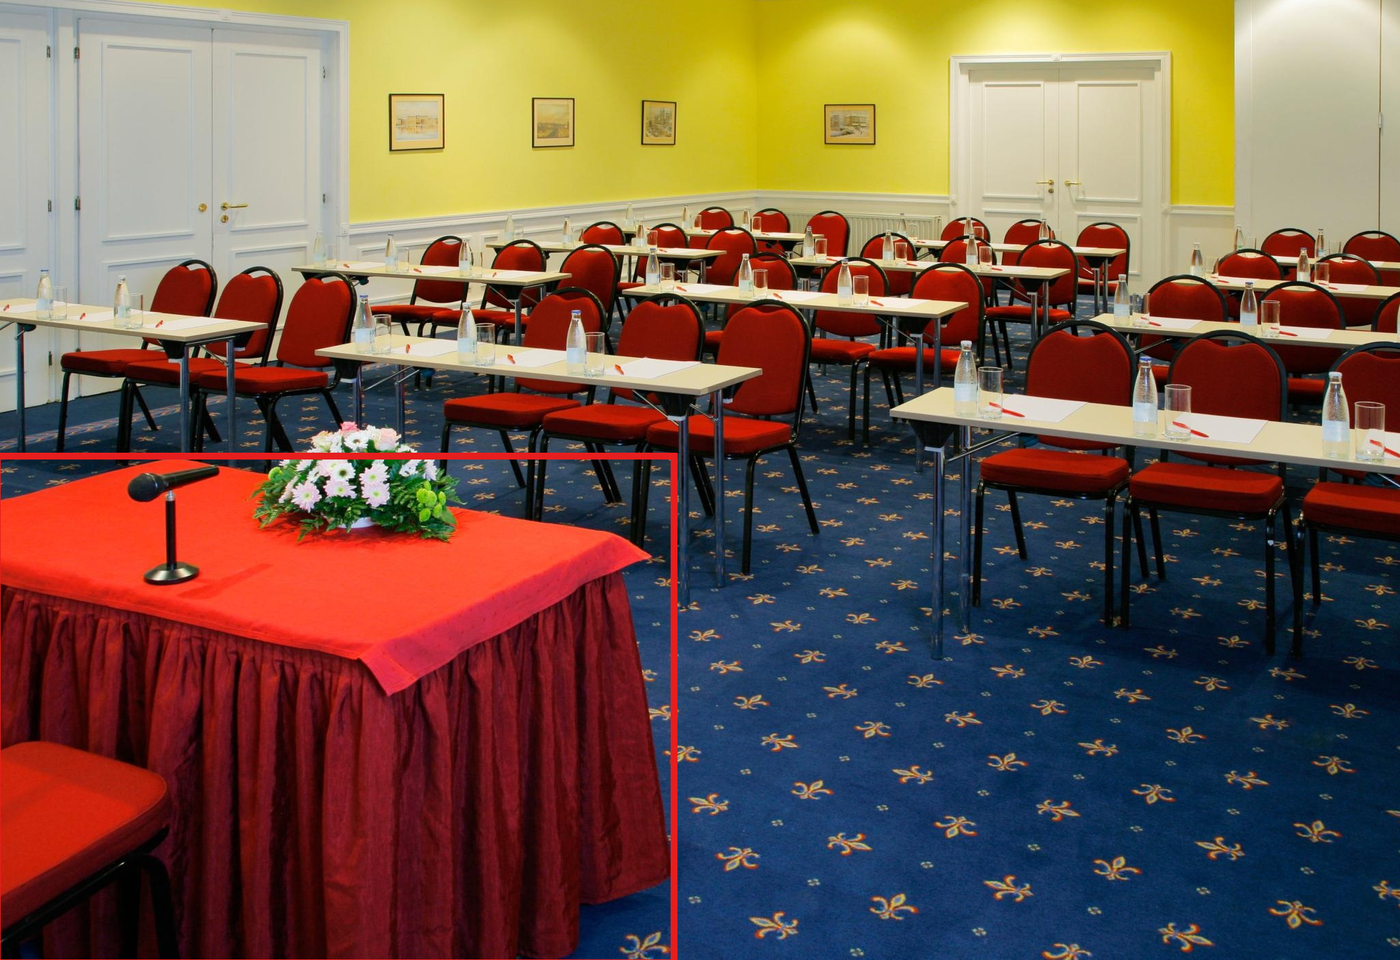
\includegraphics[width=\linewidth]{qualitative_example.png}
  \end{minipage}\hfill
  \begin{minipage}[c]{0.50\linewidth}
    \centering
    \begin{tikzpicture}[font=\footnotesize,
        card/.style={rounded corners=3pt, draw=#1!75, fill=#1!12, line width=0.8pt,
                     inner sep=4pt, text width=5cm, align=left}]
      \node[card=violet] (a) {\textbf{\textcolor{violet!65!black}{Socially Forbidden}} (Claude): ``a skirted speaker's podium''};
      \node[card=orange, below=3pt of a] (b) {\textbf{\textcolor{orange!80!black}{Socially Awkward}} (Gemini): ``a decorated presentation table''};
      \node[card=teal, below=3pt of b] (c) {\textbf{\textcolor{teal!60!black}{Object Non-functional}} (GPT-5.5, Llama): ``a table, not a seat''};
    \end{tikzpicture}
  \end{minipage}
  \caption{\textbf{Agreement on \emph{whether}, divergence on \emph{why}.} A binary can/cannot label scores these four judgments identically. The typed taxonomy exposes that the models disagree on the \emph{reason}, even along the subtle Forbidden-vs-Awkward social axis.}
  \label{fig:qualitative}
\end{figure}

\subsection{Chance-Corrected Agreement and Label Priors}
\label{sec:kappa}

Raw agreement rates flatter the consensus because the label space is skewed.
Table~\ref{tab:kappa} reports chance-corrected statistics for both selection strategies.
Agreement drops to \emph{slight} (area-ranked, Fleiss $\kappa=0.138$) or \emph{fair} (concept-targeted, $\kappa=0.246$) on the Landis--Koch scale.
Under area-ranking the 3-way $\kappa$ ($0.112$) is even lower than the 7-way ($0.138$): once chance is removed, the models do not agree on the coarse verdict any more than on the fine one there.
The whether/why asymmetry survives in conditional form: given that two models both flag an exception, they name the same type only $59.4\%$ (area) and $43.7\%$ (concept) of the time.

\begin{table}[t]
  \centering
  \footnotesize
  \caption{Chance-corrected agreement over the four standard VLMs ($K=3$). Fleiss $\kappa$, Krippendorff $\alpha$ (nominal), and mean pairwise Cohen $\kappa$, on the 7-way labels and the 3-way collapse. \emph{Type|both-exc.} = probability that two models naming an exception name the \emph{same} type. Corrected agreement is slight to fair everywhere.}
  \label{tab:kappa}
  \begin{tabular}{lcccccc}
    \toprule
    Strategy & Raw pair.\ (7) & Fleiss $\kappa_7$ & Fleiss $\kappa_3$ & Kripp.\ $\alpha_7$ & Cohen $\bar\kappa_7$ & Type$\vert$both-exc. \\
    \midrule
    SAM~2 (area)    & 0.360 & 0.138 & 0.112 & 0.138 & 0.167 & 0.594 \\
    SAM~3 (concept) & 0.462 & 0.246 & 0.340 & 0.247 & 0.263 & 0.437 \\
    \bottomrule
  \end{tabular}
\end{table}

\paragraph{Label priors, not scenes, drive much of the dissent.}
The per-model marginal label distributions expose a mechanism the consensus table hides.
Under area-ranking, Gemini assigns Object Non-functional to $5.5\%$ of pairs while the other three assign it $41$--$56\%$, preferring Firmly-Negative ($47.1\%$) and Physical Obstacle ($18.4\%$) instead.
Llama emits Dangerous and Socially Awkward almost never ($0.1\%$ each), and GPT-5.5 emits Socially Awkward on $0.4\%$.
Gemini's outlier status in Table~\ref{tab:main} is therefore largely a clash of type priors rather than per-scene dissent, and each model brings its own systematic bias about \emph{which} exception type the world contains.
A tie-free typicality score (mean agreement with the other three, no majority needed) reproduces the consensus ordering while using all $3{,}342$ pairs, so the $27.6\%$ of pairs the strict majority discards as 2--2 ties do not distort the ranking, they only hide how weak the majority is.

\paragraph{More voters do not recover consensus.}
A four-model panel is small enough that ties could plausibly be an artifact of the panel size, and all four models are closed APIs whose weights may change.
We therefore replay the \emph{identical} committed regions to the two open-weight variants of Sec.~\ref{sec:cot_ablation} and rescore the six-model pool.
Adding voters does what it should to the ties: the fraction of pairs with no strict majority falls from $27.6\%$ to $18.6\%$ under area-ranking and from $20.0\%$ to $16.8\%$ under concept-targeting.
Chance-corrected agreement nonetheless falls rather than rises, from $\kappa_7=0.138$ to $0.126$ (area) and from $0.246$ to $0.178$ (concept).
Breaking ties is not the same as finding consensus, and the additional independent voters expose more typed disagreement rather than less.
The open models also reproduce the prior-driven mechanism in a sharper form: the Instruct variant never emits Socially Awkward at all, and the Thinking variant assigns Object Non-functional to $74.7\%$ of area-ranked pairs.
Because these are open weights the replayed predictions are a frozen, reproducible snapshot, which the closed-API results of Table~\ref{tab:kappa} cannot offer.

\subsection{Region Budget and Selection}
\label{sec:ablations}

Concept-targeting (Table~\ref{tab:selection}) raises inter-model agreement markedly (pairwise $+0.10$, 4-way $+0.16$). 
Models agree far more on affordance-relevant objects than on arbitrarily large ones. 
But the same concept-targeting \emph{lowers} the exception rate ($0.62\!\to\!0.34$): area-ranking mostly returns large background objects that do not afford the action, whereas concept-targeting surfaces the objects that genuinely do, which are predominantly \emph{Positive}.
It thus trades exception coverage for reliability.

\begin{table}[t]
  \centering
  \footnotesize
  \caption{Area-ranked SAM~2 vs.\ concept-targeted SAM~3 at $K=3$ (agreement: higher is better). \emph{Exc.\ rate} = fraction of selected pairs in an exception category (2--6). Concept-targeting raises agreement but lowers the exception rate. It surfaces affordance-relevant, mostly \emph{Positive} objects.}
  \label{tab:selection}
  \begin{tabular}{lccc}
    \toprule
    & Pairwise agr.\ $\uparrow$ & 4-way agr.\ $\uparrow$ & Exc.\ rate \\
    \midrule
    SAM~2 (area-ranked)     & 0.360 & 0.072 & 0.615 \\
    SAM~3 (concept-targeted) & 0.462 & 0.236 & 0.339 \\
    \midrule
    $\Delta$ (concept $-$ area) & $+0.102$ & $+0.164$ & $-0.276$ \\
    \bottomrule
  \end{tabular}
\end{table}

\subsection{Does Consensus Track Correctness?}
\label{sec:consensus}

Experiment~B treats agreement as a reliability proxy, and Experiment~A's ground truth lets us test what that proxy is worth.
We score the majority vote of the four standard models as a fifth system on all $13{,}512$ labelled pairs, resolving tied votes either by exclusion or toward the most severe code, the same convention ADE-Affordance uses for annotator ties (Table~\ref{tab:ensemble}).

\begin{table}[t]
  \centering
  \footnotesize
  \caption{Majority-vote ensemble of the four standard VLMs vs.\ the best single model on Experiment~A. \emph{Detect}/\emph{Type} as in Table~\ref{tab:reasoning}. Ties (21.2\% of pairs) are dropped or resolved to the most severe code. The ensemble beats no column of the best single model.}
  \label{tab:ensemble}
  \begin{tabular}{lccccc}
    \toprule
    System & mAcc-7 & mAcc-3 & Detect & Type & $n$ \\
    \midrule
    Best single (Claude Sonnet 5)      & \textbf{0.289} & 0.504 & \textbf{0.763} & \textbf{0.256} & 13{,}512 \\
    Ensemble (ties dropped)            & 0.279 & \textbf{0.525} & 0.431 & 0.163 & 10{,}650 \\
    Ensemble (ties $\to$ most severe)  & 0.279 & 0.516 & 0.554 & 0.192 & 13{,}512 \\
    \bottomrule
  \end{tabular}
\end{table}

The ensemble beats no metric of the best single model, and on typed exceptions it destroys that model's advantage: majority voting drags Claude's exception detection from $0.763$ to $0.554$ because the vote pulls judgments toward the shared prior rather than toward the ground truth.
The same data quantify the paper's central caveat.
The four models agree with each other far more than any of them agrees with the labels: mean inter-model Cohen $\kappa$ is $0.214$ against a mean model--ground-truth $\kappa$ of $0.077$, a factor of $2.8$ ($0.359$ vs.\ $0.307$ raw).
Consensus in this setting rewards typicality, not correctness.
The two findings triangulate: the model most central in Experiment~B's exception consensus (GPT-5.5, $83.5\%$) is the \emph{least} accurate exception detector against ground truth ($0.233$), while the best detector (Claude, $0.763$) is repeatedly outvoted.

\subsection{Reasoning Model Analysis}
\label{sec:reasoning}

On the ADE-Affordance exception instances (codes 2--6), we compare the chain-of-thought model o4-mini against the four standard VLMs on the \emph{type}-of-constraint judgment and explanation quality (Table~\ref{tab:reasoning}).
The question is deliberately narrow: not whether reasoning raises overall accuracy, but whether it improves the harder fine-grained attribution. 
o4-mini is reported only against ground truth here.

\begin{table}[t]
  \centering
  \footnotesize
  \caption{Typed exception attribution on the 579 exception instances (codes 2--6): \emph{detection} (any exception, 3-way mAcc), exact \emph{type} (7-way mAcc), both with 95\% image-cluster bootstrap CIs, and explanation METEOR. o4-mini is chain-of-thought, while the rest are standard. Best in \textbf{bold}.}
  \label{tab:reasoning}
  \begin{tabular}{lccc}
    \toprule
    Model & Detect $\uparrow$ & Type $\uparrow$ & METEOR $\uparrow$ \\
    \midrule
    GPT-5.5             & 0.233\,{\scriptsize[.173,\,.296]} & 0.110\,{\scriptsize[.059,\,.153]} & 0.051 \\
    Claude Sonnet 5     & \textbf{0.763}\,{\scriptsize[.710,\,.814]} & \textbf{0.256}\,{\scriptsize[.213,\,.303]} & \textbf{0.168} \\
    Gemini 3.5 Flash    & 0.551\,{\scriptsize[.495,\,.604]} & 0.180\,{\scriptsize[.140,\,.213]} & 0.126 \\
    Llama 4 Maverick    & 0.371\,{\scriptsize[.313,\,.428]} & 0.128\,{\scriptsize[.086,\,.168]} & 0.080 \\
    \midrule
    o4-mini (reasoning) & 0.701\,{\scriptsize[.654,\,.748]} & 0.229\,{\scriptsize[.189,\,.269]} & 0.137 \\
    \bottomrule
  \end{tabular}
\end{table}

Explicit reasoning helps but does not dominate: o4-mini detects and types exceptions far more often than three of the four standard models and writes better explanations (METEOR $0.137$ vs.\ the $0.106$ standard-model average), yet Claude Sonnet~5's standard, non-reasoning inference matches or exceeds it on all three metrics.
Chain-of-thought reliably lifts the weaker models, but a sufficiently strong standard model rivals it.
Explicit reasoning is sufficient but not necessary here.

\subsection{Same-Weights Reasoning Ablation}
\label{sec:cot_ablation}

The comparison above confounds reasoning with model identity: o4-mini differs from the four standard models in training data and scale as well as in chain-of-thought.
The open-weight pair removes that confound.
Qwen3-VL-8B-Instruct and Qwen3-VL-8B-Thinking share a base model, so any difference between them is attributable to the reasoning trace alone.
Both are run on the same 579 exception instances under identical serving conditions.
The Thinking variant returns no parseable answer on one instance, and all numbers below are computed on the $578$ instances answered by both variants, with the difference between them bootstrapped over image clusters (Table~\ref{tab:cot}).

\begin{table}[t]
  \centering
  \footnotesize
  \caption{Same-weights chain-of-thought ablation on the $578$ exception instances answered by both variants. Detection and type as in Table~\ref{tab:reasoning}, with 95\% image-cluster bootstrap CIs. The $\Delta$ row is the paired difference with its own bootstrap CI. Reasoning improves detection but not typing.}
  \label{tab:cot}
  \begin{tabular}{lccc}
    \toprule
    Variant & Detect $\uparrow$ & Type $\uparrow$ & METEOR $\uparrow$ \\
    \midrule
    Qwen3-VL-8B-Instruct & 0.649\,{\scriptsize[.593,\,.701]} & 0.190\,{\scriptsize[.145,\,.231]} & 0.148 \\
    Qwen3-VL-8B-Thinking & \textbf{0.709}\,{\scriptsize[.660,\,.755]} & \textbf{0.215}\,{\scriptsize[.163,\,.260]} & \textbf{0.162} \\
    \midrule
    $\Delta$ (Thinking $-$ Instruct) & $+0.061$\,{\scriptsize[+.016,\,+.111]} & $+0.025$\,{\scriptsize[$-$.043,\,+.094]} & $+0.014$ \\
    \bottomrule
  \end{tabular}
\end{table}

Chain-of-thought buys detection, not attribution.
The reasoning trace raises exception detection by $+0.061$, a gain whose bootstrap CI excludes zero, while the typed judgment improves by only $+0.025$ with a CI spanning zero.
With weights held fixed, reasoning therefore reproduces exactly the asymmetry this paper reports across models: it helps decide \emph{whether} an action is blocked and leaves \emph{why} unresolved.
This also confirms that the asymmetry is not an artifact of comparing different model families.

\begin{table}[t]
  \centering
  \footnotesize
  \setlength{\tabcolsep}{4pt}
  \caption{Where the reasoning trace changes the typed judgment, on the same $578$ instances. Each row splits the ground-truth exceptions of one axis into exact type, right axis but wrong type, wrong axis, and missed. Reasoning redistributes typing across axes rather than uniformly improving it.}
  \label{tab:cotaxis}
  \begin{tabular}{llcccc}
    \toprule
    Axis & Variant & Exact $\uparrow$ & Right axis & Wrong axis & Missed $\downarrow$ \\
    \midrule
    Functional  & Instruct & \textbf{0.333} & 0.257 & 0.012 & 0.398 \\
    ($n{=}171$) & Thinking & 0.158 & \textbf{0.409} & 0.158 & \textbf{0.275} \\
    \midrule
    Social      & Instruct & 0.003 & 0.003 & 0.636 & 0.358 \\
    ($n{=}332$) & Thinking & \textbf{0.063} & \textbf{0.063} & \textbf{0.524} & \textbf{0.349} \\
    \midrule
    Danger      & Instruct & 0.093 & --- & 0.693 & 0.213 \\
    ($n{=}75$)  & Thinking & \textbf{0.413} & --- & \textbf{0.520} & \textbf{0.067} \\
    \bottomrule
  \end{tabular}
\end{table}

The aggregate null hides a systematic redistribution (Table~\ref{tab:cotaxis}).
Without the reasoning trace the model has effectively abandoned two of the three constraint axes: it emits a social code on $2$ of $578$ instances and types only $9.3\%$ of dangerous instances correctly, funnelling almost every detected exception into the functional codes.
The reasoning trace reverses this.
Social codes rise from $2$ to $57$ emissions, exact social typing from $0.003$ to $0.063$, and exact danger typing from $0.093$ to $0.413$ with missed danger instances falling from $0.213$ to $0.067$.
The gains are paid for on the functional axis, where exact typing falls from $0.333$ to $0.158$, although the predictions remain on the correct axis: right-axis attribution rises from $0.257$ to $0.409$, so the model still recognizes a functional constraint and merely picks the wrong functional code.
Net typed accuracy barely moves because these movements cancel.

What reasoning changes here is the label prior rather than the discrimination.
The Instruct variant behaves as if most of the taxonomy did not exist, and the reasoning trace restores access to the neglected categories without making the model better at choosing among them.
This is the same prior-driven mechanism identified in Sec.~\ref{sec:kappa} for the frontier models, observed within a single set of weights and switched on and off by inference mode alone.
It also tempers a natural reading of Sec.~\ref{sec:reasoning}: chain-of-thought does not simply add typed competence, and a headline accuracy that hardly moves can conceal a wholesale reallocation of the model's typed predictions.

\subsection{Semantic Explanation Quality}
\label{sec:semantic}

The $n$-gram scores of Table~\ref{tab:expA} were computed over all ground-truth exceptions, so a model that misses an exception contributes an empty explanation and scores zero.
They therefore conflate \emph{detection} with \emph{explanation quality}.
Table~\ref{tab:semantic} separates the two with the semantic measures of Sec.~\ref{sec:method}, reporting each both over all 579 exceptions (empty candidates count as zero, the convention of Table~\ref{tab:expA}) and over only the rows where the model wrote an explanation.

\begin{table}[t]
  \centering
  \footnotesize
  \setlength{\tabcolsep}{4.5pt}
  \caption{Semantic explanation quality on the 579 ground-truth exceptions. \emph{all} counts missed exceptions as zero (the convention behind Table~\ref{tab:expA}); \emph{det.} conditions on the model having written an explanation ($n$ rows). \emph{cos exact} / \emph{cos w-axis} split the detected rows by whether the predicted type was exactly right or on the wrong constraint axis. Best of the four standard models per column \textbf{bold}. The open-weight pair is scored on the same references and, for Thinking, over its $578$ answered instances.}
  \label{tab:semantic}
  \begin{tabular}{lrccccccc}
    \toprule
    & & \multicolumn{2}{c}{Cosine} & \multicolumn{2}{c}{NLI entail.} & BSc-F1 & \multicolumn{2}{c}{Cosine by type} \\
    \cmidrule(lr){3-4}\cmidrule(lr){5-6}\cmidrule(lr){8-9}
    Model & $n$ & all & det. & all & det. & det. & exact & w-axis \\
    \midrule
    GPT-5.5             & 135 & 0.109 & 0.468 & 0.071 & 0.305 & 0.873 & 0.463 & 0.466 \\
    Claude Sonnet 5     & 442 & \textbf{0.387} & \textbf{0.507} & \textbf{0.258} & \textbf{0.338} & 0.870 & \textbf{0.520} & \textbf{0.497} \\
    Gemini 3.5 Flash    & 319 & 0.228 & 0.413 & 0.112 & 0.203 & 0.871 & 0.389 & 0.426 \\
    Llama 4 Maverick    & 215 & 0.158 & 0.425 & 0.064 & 0.172 & \textbf{0.880} & 0.410 & 0.421 \\
    \midrule
    o4-mini (reasoning) & 406 & 0.319 & 0.455 & 0.150 & 0.213 & 0.882 & 0.463 & 0.450 \\
    \midrule
    Qwen3-VL-8B-Instr.  & 376 & 0.313 & 0.482 & 0.127 & 0.195 & 0.882 & 0.500 & 0.483 \\
    Qwen3-VL-8B-Think.  & 410 & 0.343 & 0.484 & 0.174 & 0.245 & 0.881 & 0.473 & 0.479 \\
    \bottomrule
  \end{tabular}
\end{table}

Two conclusions follow.
First, the apparent explanation-quality gap between models is mostly a detection gap.
Under the all-rows convention the models span $0.109$--$0.387$ in cosine similarity, mirroring the METEOR ordering of Table~\ref{tab:expA}, but conditioned on detection the span collapses to $0.413$--$0.507$ and GPT-5.5 moves from last to second.
Once a model recognizes that an exception applies, all five write explanations of broadly similar semantic quality.
Second, the typed label and the free-text reason are partly decoupled.
Explanations attached to a wrong-axis type are almost as aligned with the human references as those attached to the exact type (Claude: $0.497$ vs.\ $0.520$ cosine), and for Gemini and GPT-5.5 the wrong-axis rows score marginally \emph{higher}.
The right-axis-wrong-type rows carry the strongest entailment scores of all, although their per-model counts are small ($8$--$54$ rows).
Models thus often perceive the correct reason but file it under the wrong code, so part of the typed divergence of Sec.~\ref{sec:kappa} is a taxonomy-mapping failure rather than a perception failure.
This substantiates the claim that near-zero $n$-gram scores reflect phrasing variety rather than wrong content, with one amendment: they also reflect missed detections, which no text metric should be asked to absorb.
BERTScore~F1 is reported for completeness but compresses to $0.87$--$0.88$ for every model on detected rows, and discriminates little at this granularity.

The open-weight pair extends both conclusions beyond the closed models and adds a third.
Conditioned on detection they fall squarely inside the band the frontier models occupy ($0.482$ and $0.484$ cosine, against a $0.413$--$0.507$ span), which is further evidence that explanation quality converges once a model recognizes the exception at all.
The label--text decoupling recurs in the Thinking variant in its strongest form: its wrong-axis explanations score marginally \emph{higher} than its exact-type ones ($0.479$ vs.\ $0.473$ cosine), and its right-axis rows lead on entailment by a wide margin ($0.322$ vs.\ $0.233$).
Reasoning traces do not repair the mapping from a correctly perceived reason to the correct code, which is the same conclusion Sec.~\ref{sec:cot_ablation} reaches from the typed labels.

The third point concerns where the remaining headroom lies.
Qwen3-VL-8B-Thinking ranks second of all seven models on explanation semantics under the all-rows convention ($0.343$ cosine and $0.174$ entailment, behind only Claude) and second on METEOR ($0.162$ vs.\ Claude's $0.168$), while ranking third on typed accuracy and using $8$B open weights on a single consumer GPU.
Its free text is therefore a better guide to what it understood than its typed label is.
Read together with Sec.~\ref{sec:remap}, where a text-only mapper recovers accuracy from Claude's explanations, this locates the bottleneck in the mapping from reason to code rather than in the perception or the language, and it suggests that the mapping is what a purpose-built model should learn.

The consequence field repeats both patterns and adds one.
Conditioned on detection, consequence cosine similarity spans $0.452$--$0.560$ (all-rows: $0.130$--$0.405$), slightly \emph{higher} than for explanations, so models converge more on what would happen than on why it is blocked.
The label--text decoupling persists: o4-mini's wrong-axis consequences align better with the references than its exact-type ones ($0.570$ vs.\ $0.557$ cosine), and Claude's nearly match ($0.521$ vs.\ $0.550$).
Entailment scores are uniformly lower than for explanations ($0.084$--$0.224$ detected), reflecting that a scene admits many distinct valid outcomes but fewer valid reasons.

\subsection{LLM-Judge Corroboration and a Validity Audit}
\label{sec:judge}

We add an LLM judge as an independent view on explanation quality, and---because judge scores are only as good as the judge---audit the judge itself.
For every detected exception, a held-out model (Gemini~3.1~Flash-Lite, deliberately \emph{not} one of the evaluated models, to avoid self-preference) sees the action, the reference explanations, and the model explanation, and rules whether they express the \emph{same} reason, are \emph{partially related}, or give a \emph{different} reason (Table~\ref{tab:judge}).

\begin{table}[t]
  \centering
  \footnotesize
  \setlength{\tabcolsep}{5pt}
  \caption{LLM-judge reason-match on detected exceptions: fraction judged \emph{same} / \emph{different} reason vs.\ the human references, and the \emph{same}-rate split by whether the predicted type was exact or on the wrong axis. The judge's model ranking matches the semantic metrics of Table~\ref{tab:semantic}.}
  \label{tab:judge}
  \begin{tabular}{lrcccc}
    \toprule
    Model & $n$ & same $\uparrow$ & different $\downarrow$ & same$\vert$exact & same$\vert$wrong-axis \\
    \midrule
    GPT-5.5             & 135 & 0.385 & 0.570 & 0.450 & 0.358 \\
    Claude Sonnet 5     & 442 & \textbf{0.507} & \textbf{0.430} & \textbf{0.685} & \textbf{0.449} \\
    Gemini 3.5 Flash    & 319 & 0.329 & 0.536 & 0.286 & 0.350 \\
    Llama 4 Maverick    & 215 & 0.200 & 0.730 & 0.220 & 0.194 \\
    \midrule
    o4-mini (reasoning) & 406 & 0.288 & 0.645 & 0.400 & 0.259 \\
    \bottomrule
  \end{tabular}
\end{table}

Two things follow, one confirmatory and one cautionary.
First, the judge \emph{independently reproduces} the ordering the semantic metrics gave (Claude $>$ GPT-5.5 $>$ Gemini $>$ o4-mini $>$ Llama on \emph{same}-reason), so the explanation-quality picture is not an artifact of a single metric family.
It also sharpens the reason-first story: for most models the \emph{same}-rate is higher on exact-type rows than on wrong-axis rows (Claude $0.685$ vs.\ $0.449$), a wider gap than the embedding cosine showed---so mistyped detections carry the right reason \emph{less} often than surface similarity implied, though still substantially (wrong-axis \emph{same}-rate $0.19$--$0.45$, and for Gemini even higher on wrong-axis rows).

Second, the audit shows why the judge must not be treated as ground truth.
Re-judging identical inputs is perfectly stable ($1.000$; the judge is deterministic at temperature~$0$), but reversing the reference order or applying a meaning-preserving surface rewrite (lowercasing, stripping a final period, prepending ``I think'') each flip \textbf{$11.3\%$} of verdicts (stability $0.887$).
The judge is thus \emph{reliable but not valid}: perfectly self-consistent, yet one verdict in nine is fragile to perturbations that cannot change whether two texts share a reason.
This is the field's ``reliability without validity'' concern made concrete on our task, and it is the reason we report the judge only alongside the reference-based semantic metrics rather than as a standalone score.

\subsection{A Reason-First Probe: Re-Mapping Reasons to Types}
\label{sec:remap}

If models often name the right reason under the wrong code, a mapper from reason text to type should recover accuracy without touching the models.
We test this directly.
A logistic classifier over sentence embeddings is trained on the ADE-Affordance \emph{train} split ($21{,}119$ explanation--code pairs, codes 2--6) and applied to the frontier models' own explanations on Experiment~A: wherever a model flagged an exception, its code is replaced by the mapper's prediction from the model's sentence (Table~\ref{tab:remap}).

\begin{table}[t]
  \centering
  \footnotesize
  \caption{Re-mapping model explanations to exception types with a text-only mapper trained on the ADE-Affordance train split. \emph{Type} as in Table~\ref{tab:reasoning}; \emph{ceiling} scores every detected exception as correctly typed. The mapper lifts the model with the strongest explanations by $37\%$ relative and leaves the others unchanged or worse.}
  \label{tab:remap}
  \begin{tabular}{lcccc}
    \toprule
    Model & Type (label) & Type (re-mapped) & Detection ceiling & re-mapped rows \\
    \midrule
    GPT-5.5             & 0.110 & 0.101 & 0.258 & 135 \\
    Claude Sonnet 5     & 0.256 & \textbf{0.350} & 0.786 & 442 \\
    Gemini 3.5 Flash    & 0.180 & 0.183 & 0.552 & 319 \\
    Llama 4 Maverick    & 0.128 & 0.109 & 0.390 & 215 \\
    \midrule
    o4-mini (reasoning) & 0.229 & 0.237 & 0.718 & 406 \\
    \bottomrule
  \end{tabular}
\end{table}

Three observations.
First, the probe works exactly where the diagnosis predicts: Claude, whose explanations align best with the references (Table~\ref{tab:semantic}), gains $37\%$ relative ($0.256\!\to\!0.350$) --- a new best Type score obtained purely by re-reading the model's own words.
Second, the gain tracks explanation quality: models with weaker text (GPT-5.5, Llama) gain nothing or lose slightly, so the mapper cannot rescue reasons that were never articulated.
Third, the text-only route saturates quickly: the same mapper reaches only $0.374$ on held-out \emph{human} annotator explanations (zero-shot embedding baseline: $0.215$, chance $0.2$), and Claude's re-mapped $0.350$ sits close to that ceiling.
The reason text alone does not determine the type: ``it is a table, not a seat'' is Firmly-Negative or Object-Non-functional depending on what the image shows.
Typing therefore needs the reason \emph{and} the pixels, which motivates jointly trained reason-first models rather than post-hoc text mapping.


% ============================================================
\section{Discussion and Conclusion}
\label{sec:discussion}

\paragraph{Frontier models agree on \emph{whether}, not on \emph{why}.}
Agreement across the four frontier models is modest and highly uneven: unanimity is only $7.2\%$ (vs.\ ${\sim}0.3\%$ by chance), and it concentrates on \emph{Positive} affordances while nearly vanishing on the typed exceptions ($34.5\%$ vs.\ $\!6.3\%$).
They concur that an action \emph{is} possible but assign different \emph{reasons} when it is not.
The audit sharpens this picture in three ways.
First, chance correction shows the consensus is thinner than raw rates suggest (Fleiss $\kappa$ $0.14$--$0.25$), and the whether/why gap is best stated conditionally: models that both flag an exception still disagree on its type roughly half the time (Sec.~\ref{sec:kappa}).
Second, much of the typed disagreement is systematic rather than scene-specific: each model carries its own prior over exception types, from Gemini's aversion to Object Non-functional to Llama's near-total refusal of Dangerous.
Third, the agreement signal must not be read as correctness: models agree with each other $2.8\times$ more than with the labels (chance-corrected), the majority vote loses to the best single model on every metric, and the most typical model in the exception consensus is the least accurate exception detector against ground truth (Sec.~\ref{sec:consensus}).
Fourth, the typed disagreement overstates the semantic disagreement: explanations attached to the wrong type are nearly as aligned with the human references as those attached to the right one, so models often perceive the correct reason and file it under the wrong code (Sec.~\ref{sec:semantic}), a reading an independent LLM judge corroborates while its own perturbation audit warns against over-trusting it (Sec.~\ref{sec:judge}).
Fifth, the asymmetry is not an artifact of comparing model families: holding weights fixed and switching only the reasoning trace on and off improves detection significantly while leaving typed accuracy unchanged (Sec.~\ref{sec:cot_ablation}).
That ablation also shows the label-prior mechanism operating within a single model, where reasoning restores access to constraint axes the base variant had all but abandoned without improving the choice among them.
Typed attribution is where frontier VLMs diverge, and where their consensus is least trustworthy.

\paragraph{Limitations.}
ADE ground truth covers only three of our six actions, so \texttt{cut}, \texttt{throw}, and \texttt{ride} are evaluated ground-truth-free.
Furthermore, inter-model agreement is a reliability signal, not a measure of correctness, and Sec.~\ref{sec:consensus} shows the gap is material rather than hypothetical in this setting.
The social and safety codes encode a particular normative frame --- the Awkward-vs-Forbidden boundary is culturally contestable --- and four of our models are closed, drifting API endpoints, a limitation the open-weight replays of Sec.~\ref{sec:kappa} answer only in part.
Applying the AGD20K vocabulary to ADE20K scenes also leaves some actions sparse or ill-posed: concept targeting with SAM 3 finds rideable objects in only $5$ of $200$ scenes, and \texttt{throw} yields just $1$--$2\%$ four-way agreement. 
So the weakest scores partly reflect this domain mismatch rather than model divergence alone. 
Better-matched scenes, spatial grounding, and a larger action set would strengthen generality.

\paragraph{Conclusion.}
Typing affordances by the \emph{reason} why an action is blocked cleanly separates two capabilities: judging \emph{whether} an action is possible, which today's frontier VLMs largely share, and agreeing on \emph{why} it is not, which they do not.
We hope this framing, with its annotation-free pipeline on existing data, guides future work toward models that reason not just about what can be done, but also about \emph{why it can not}.

% ---- Bibliography ----
%
% BibTeX users should specify bibliography style 'splncs04'.
% References will then be sorted and formatted in the correct style.
%
\bibliographystyle{splncs04}
\bibliography{main}
\end{document}
